\begin{figure*}[!t]
	\begin{minipage}{.49\textwidth}
		\centering
		\includegraphics[width=.7\textwidth]{images/petri.pdf}
		\caption{A sample \uswn. Labels are shown in green, $\tau$ transitions in grey, weights in magenta.}\label{fig:spn}
	\end{minipage}\hfill \begin{minipage}{.49\textwidth}\centering
		\includegraphics[width=.8\textwidth]{images/rg.pdf}
		\caption{Reachability graph $RG(N)$ of the \uswn $N$. Probabilities are shown in violet.}\label{fig:rg}
	\end{minipage}
\end{figure*} \begin{figure*}[!t]
	\begin{minipage}{.49\textwidth}\centering \includegraphics[width=.55\textwidth]{images/running_example.pdf}
		\caption{Transition graph $G_{RG(N)}$ encoding the reachability graph $RG(N)$.}\label{fig:lmc}\label{fig:orig}
	\end{minipage}\hfill \begin{minipage}{.49\textwidth}\centering \includegraphics[width=.55\textwidth]{images/closed_example.pdf}
		\caption{Transition graph $\closed{G_{RG(N)}}$ resulting from the transition graph in $G_{RG(N)}$ after $\tau$-closure.}\label{fig:closed}
	\end{minipage}
\end{figure*}
\section{Computation Pipeline}
%\begin{figure}[!t]
%	\centering
%	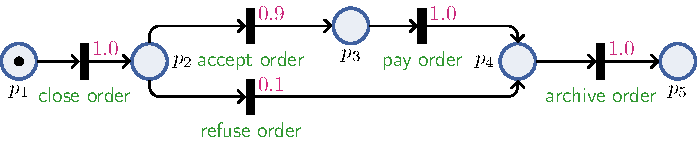
\includegraphics[width=.49\textwidth]{images/petri_tut.pdf}
%	\caption{Stochastic Workflow Net modeling our use-case scenario.}\label{fig:petri_tut}
%\end{figure}
\begin{figure}[!t]
	\centering\includegraphics[width=\textwidth]{images/pipeline}
	\caption{Proposed pipeline to assess the probabilistic trace alignment.}\label{fig:pipe}
\end{figure}

%We now describe the proposed technique for computing probabilistic trace alignments. 
Our approach (\figurename~\ref{fig:pipe}) takes as input
\begin{inparaenum}[\it (i)]
	\item a reference model represented as Stochastic Workflow Nets $\net$ or an equivalent Transition Graph $G$,
	\item a minimum, positive probability threshold $\pmin \in (0,1]$
	\item a trace $\trace$ of interest,
\end{inparaenum}
and returns a ranking over all the $\net$-traces having a probability greater than or equal to $\pmin$, based on a combined consideration of their probability values and their distance to $\trace$.